%external files that are referenced
%\externaldocument{thesis}
%\externaldocument{integration}
%%%%%%
\chapter{Supplementary material for}\label{ch:SupplIntegration}

\begin{figure}
    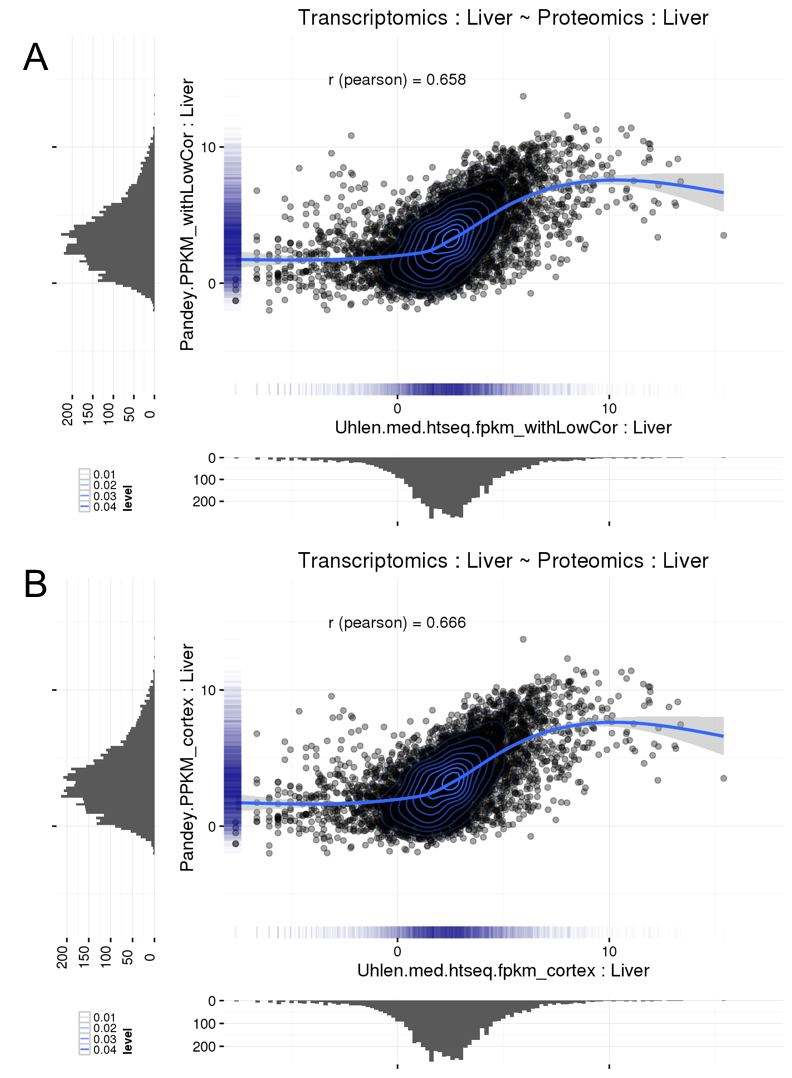
\includegraphics[scale=0.75]{integration/LiverScat}\centering
    \caption[Scatter plot between transcriptomic and proteomic
    for Liver]{\label{fig:ScatterPlotLiver}\textbf{Scatter plot between
    transcriptomic (x-axis) and proteomic (y-axis) for Liver}\\
    A| with the anticorrelated \mRNAs\ B| without the anticorrelated \mRNAs}
\end{figure}


\begin{figure}
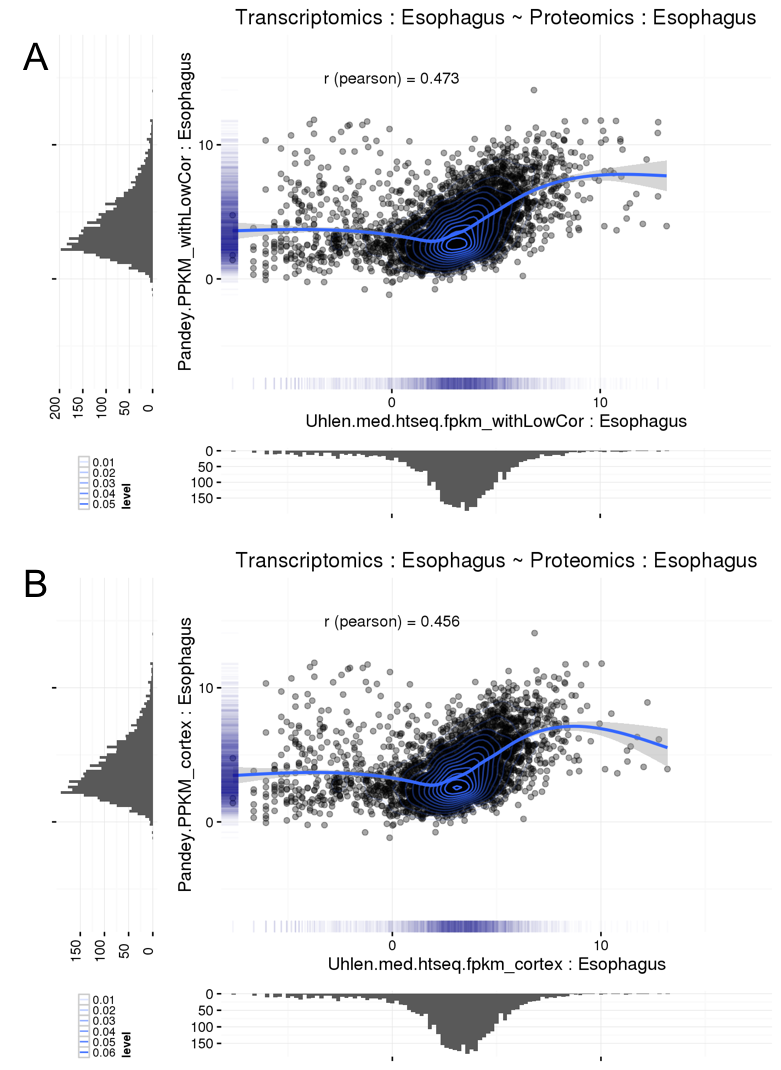
\includegraphics[scale=0.75]{integration/OesophagusScat}\centering
    \caption[Scatter plot between transcriptomic and
    proteomic for Oesophagus]{\label{fig:ScatterPlotOesophagus}\textbf{Scatter plot between
    transcriptomic (x-axis) and  proteomic (y-axis) for Oesophagus}\\
    A| with the anticorrelated \mRNAs\ B| without the anticorrelated \mRNAs}
\end{figure}


\begin{figure}
    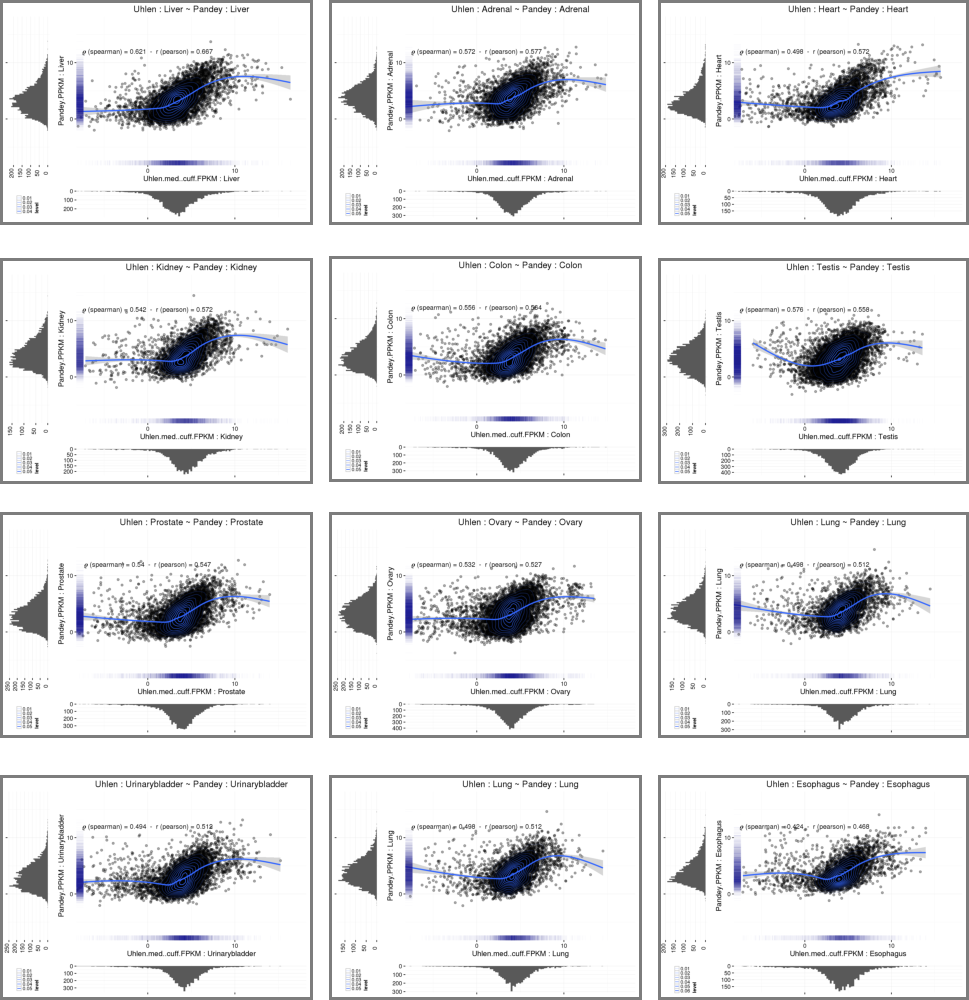
\includegraphics[scale=0.9]{integration/scatterplots.pdf}\centering
    \caption[Scatter plot between transcriptomic and
    proteomic for all tissues]{\label{fig:ScatterPlotAll}\textbf{Scatter plot between
    transcriptomic (x-axis) and  proteomic (y-axis) for all the tissues}}
\end{figure}


\begin{figure}%[!htbp]
    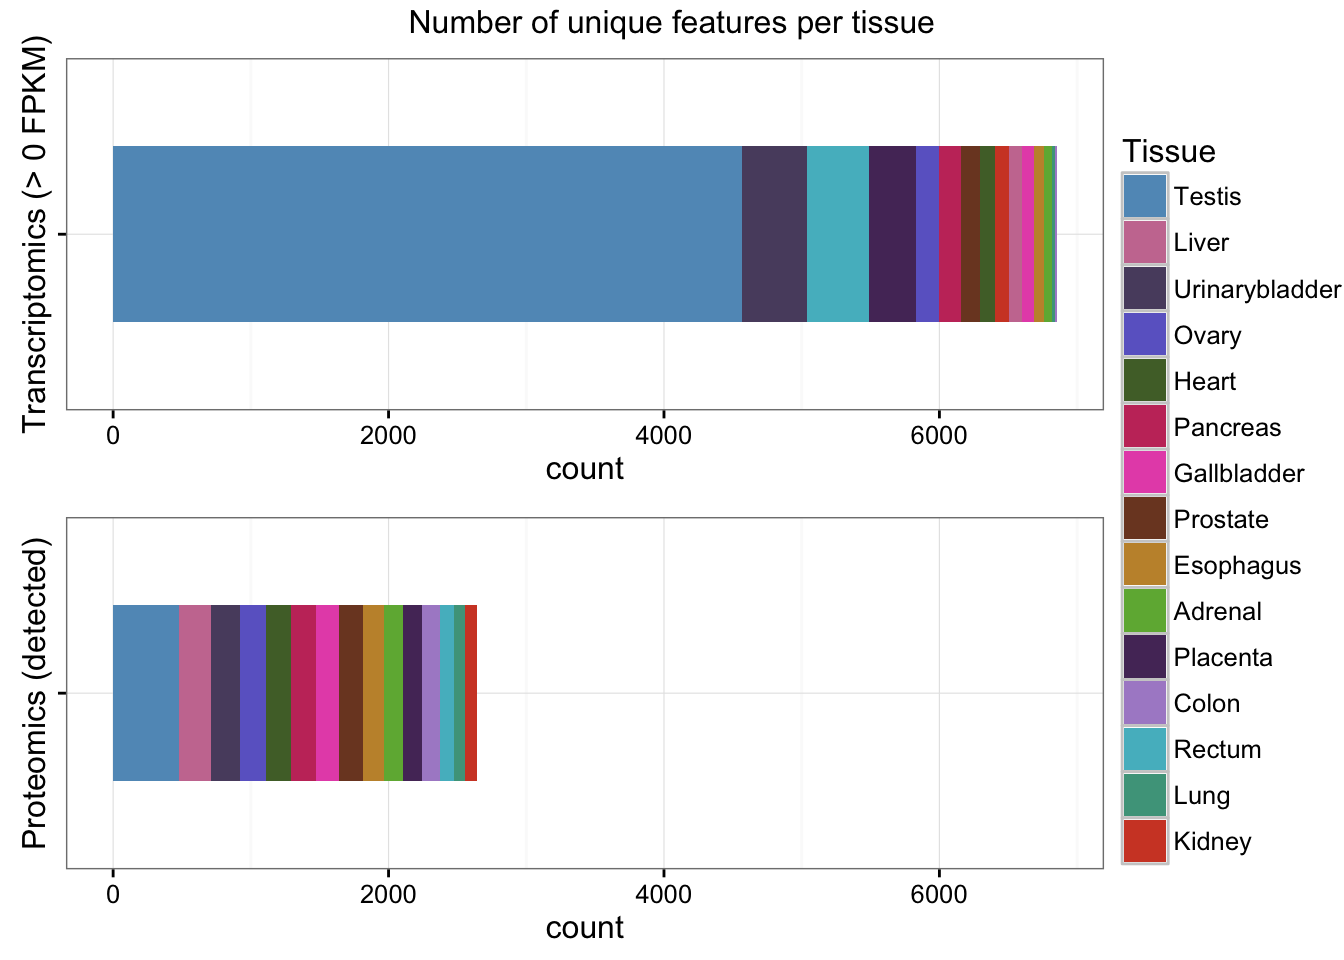
\includegraphics[scale=0.30]{integration/barPlotunique0nb}\centering
    \caption[Number of \mRNAs\ and proteins detected  only in one
    unique tissue]{\label{fig:barPlotunique0nb}\textbf{Number of
    \mRNAs\ (top) and proteins (bottom)
    that have been detected and quantified (\textgreater\ 0 \gls{FPKM} for \mRNA\
    and for proteins).}}
\end{figure}

\begin{figure}%[!htbp]
    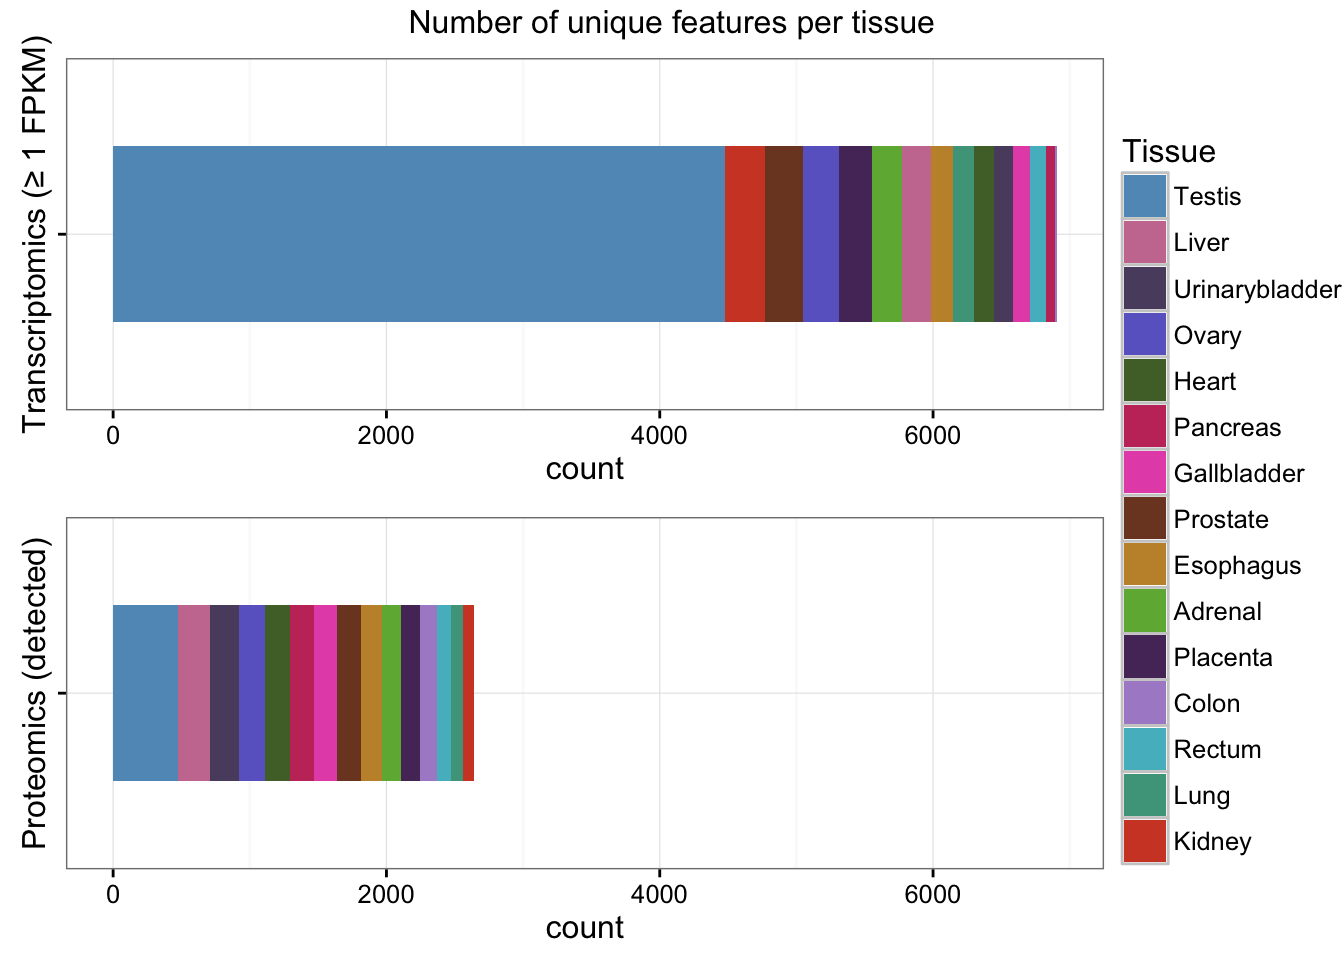
\includegraphics[scale=0.30]{integration/barPlotunique1nb}\centering
    \caption[Number of \mRNAs\ (\geq\ 1 \gls{FPKM})
    and proteins detected (at specific thresholds) only in one unique
    tissue]{\label{fig:barPlotunique1nb}\textbf{Number of
    \mRNAs\ (top) and proteins (bottom)
    that have been detected and quantified (\geq\ 1 \gls{FPKM} for \mRNA\;
    \textgreater\ 0 for proteins).} While some tissue can have consistently a higher
    specificity at proteomic and transcriptomic level, it is not true for all.}
\end{figure}



\begin{figure}%[!htbp]
    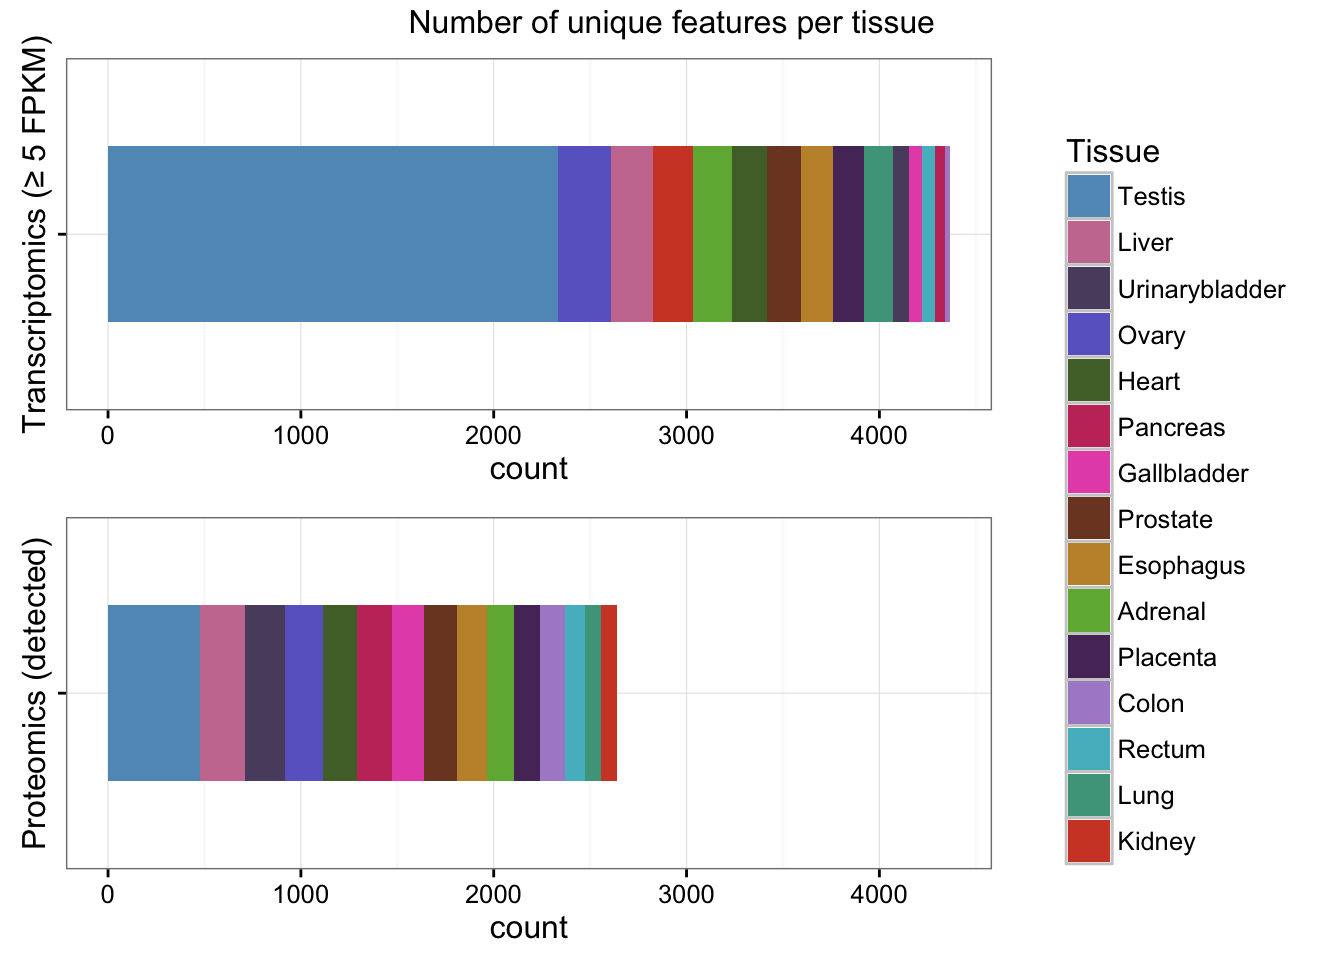
\includegraphics[scale=0.30]{integration/barPlotunique5nb}\centering
    \caption[Number of \mRNAs\ (\geq\ 5 \glspl{FPKM}) and proteins detected
    (at specific thresholds) only in one unique
    tissue]{\label{fig:barPlotunique5nb}\textbf{Number of \mRNAs\ (top)
    and proteins (bottom) that have been detected and quantified
    (\geq\ 5 \glspl{FPKM} for \mRNA\; \textgreater\ 0 for proteins).}}
\end{figure}


\begin{figure}[!htbp]
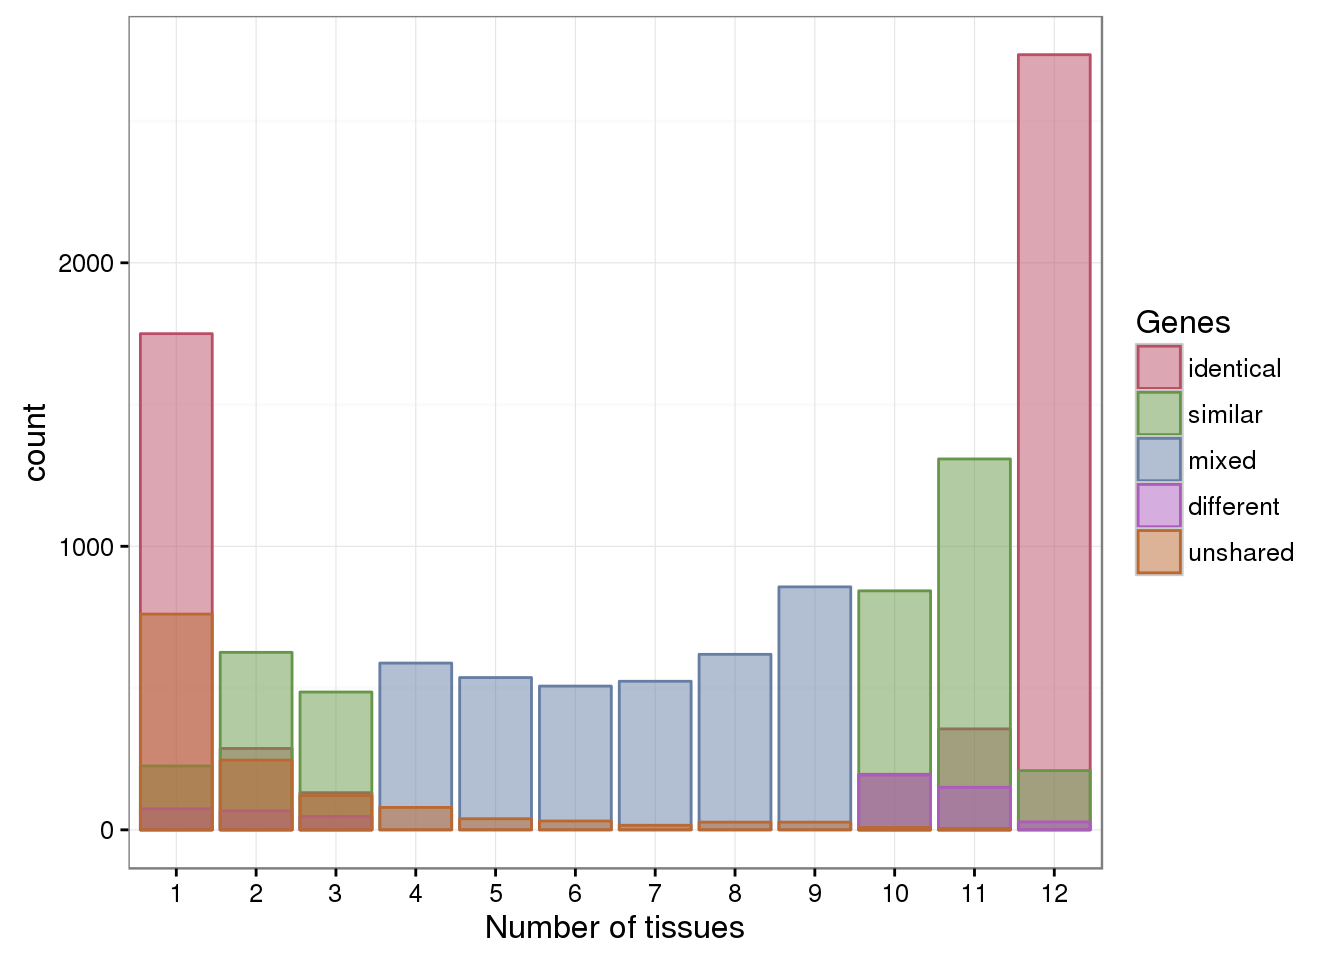
\includegraphics[scale=1]{integration/GtexUhlenAnnoBreadth}
\caption[placeHold]{\label{fig:breadthColGtexUhlen}\textbf{placeHold}}
\end{figure}




\clearpage
\pagestyle{plain}
\begin{landscape}
    \begin{longtable}{@{}llllll@{}}%[]%\centering
    \caption{Found proteins without a counterpart in the transcriptomic data}\label{tab:protNoTrans}\\
        \toprule
        Ensembl Gene ID & Description & Source & \begin{tabular}[c]{@{}l@{}}Accessing number\\  (in Source)\end{tabular} & Gene Biotype & \begin{tabular}[c]{@{}l@{}}Associated\\ Gene Name\end{tabular} \\ \midrule
        ENSG00000105371 & \begin{tabular}[c]{@{}l@{}}intercellular adhesion molecule 4 \\ (Landsteiner-Wiener blood group)\end{tabular} & \begin{tabular}[c]{@{}l@{}}HGNC\\Symbol\end{tabular} & 5347 & protein\_coding & ICAM4 \\
        ENSG00000142539 & -  & -  & - & protein\_coding & CTD-2545M3.6 \\
        ENSG00000148136 & \begin{tabular}[c]{@{}l@{}}olfactory receptor, family 13, \\ subfamily C, member 4\end{tabular} & \begin{tabular}[c]{@{}l@{}}HGNC\\ Symbol\end{tabular} & 14722 & protein\_coding & OR13C4 \\
        ENSG00000163157 & tropomodulin 4 (muscle) & \begin{tabular}[c]{@{}l@{}}HGNC\\ Symbol\end{tabular} & 11874 & protein\_coding & TMOD4 \\
        ENSG00000164708 & \begin{tabular}[c]{@{}l@{}}phosphoglycerate mutase 2 \\ (muscle)\end{tabular} & \begin{tabular}[c]{@{}l@{}}HGNC\\ Symbol\end{tabular} & 8889 & protein\_coding & PGAM2 \\
        ENSG00000166884 & \begin{tabular}[c]{@{}l@{}}olfactory receptor, family 4, \\ subfamily D, member 6\end{tabular} & \begin{tabular}[c]{@{}l@{}}HGNC\\ Symbol\end{tabular} & 15175 & protein\_coding & OR4D6 \\
        ENSG00000171396 & keratin associated protein 4--4 & \begin{tabular}[c]{@{}l@{}}HGNC\\ Symbol\end{tabular} & 16928 & protein\_coding & KRTAP4--4 \\
        ENSG00000171501 & \begin{tabular}[c]{@{}l@{}}olfactory receptor, family 1,\\ subfamily N, member 2\end{tabular} & \begin{tabular}[c]{@{}l@{}}HGNC\\ Symbol\end{tabular} & 15111 & protein\_coding & OR1N2 \\
        ENSG00000173349 & SFT2 domain containing 3 & \begin{tabular}[c]{@{}l@{}}HGNC\\ Symbol\end{tabular} & 28767 & protein\_coding & SFT2D3 \\
        ENSG00000176239 & \begin{tabular}[c]{@{}l@{}}olfactory receptor, family 51, \\ subfamily B, member 6\end{tabular} & \begin{tabular}[c]{@{}l@{}}HGNC\\ Symbol\end{tabular} & 19600 & protein\_coding & OR51B6 \\
        ENSG00000181404 & - & - & - & unprocessed\_pseudogene & XXyac-YRM2039.2 \\
        ENSG00000182346 & \begin{tabular}[c]{@{}l@{}}D-amino acid oxidase\\ activator\end{tabular} & \begin{tabular}[c]{@{}l@{}}HGNC\\ Symbol\end{tabular} & 21191 & protein\_coding & DAOA \\
        ENSG00000182591 & keratin associated protein 11--1 & \begin{tabular}[c]{@{}l@{}}HGNC\\ Symbol\end{tabular} & 18922 & protein\_coding & KRTAP11--1 \\
            ENSG00000183214 &\begin{tabular}[c]{@{}l@{}} MHC class I polypeptide-related\\ sequence A\end{tabular} & \begin{tabular}[c]{@{}l@{}}HGNC\\ Symbol\end{tabular} & 7090 & protein\_coding & MICA \\
        ENSG00000183336 & bolA family member 2 & \begin{tabular}[c]{@{}l@{}}HGNC\\ Symbol\end{tabular} & 29488 & protein\_coding & BOLA2 \\
        ENSG00000184321 & \begin{tabular}[c]{@{}l@{}}olfactory receptor, family 51,\\ subfamily J, member 1 \\ (gene/pseudogene)\end{tabular} & \begin{tabular}[c]{@{}l@{}}HGNC\\ Symbol\end{tabular} & 14856 & protein\_coding & OR51J1 \\
        ENSG00000186090 & \begin{tabular}[c]{@{}l@{}}5-hydroxytryptamine (serotonin)\\ receptor 3D, ionotropic\end{tabular} & \begin{tabular}[c]{@{}l@{}}HGNC\\ Symbol\end{tabular} & 24004 & protein\_coding & HTR3D \\
        ENSG00000187766 & keratin associated protein 10--8 & \begin{tabular}[c]{@{}l@{}}HGNC\\ Symbol\end{tabular} & 20525 & protein\_coding & KRTAP10--8 \\
        ENSG00000196101 & \begin{tabular}[c]{@{}l@{}}major histocompatibility \\complex, class II, \\ DR beta 3\end{tabular} & \begin{tabular}[c]{@{}l@{}}HGNC\\ Symbol\end{tabular} & 4951 & protein\_coding & HLA-DRB3 \\
        ENSG00000203618 & \begin{tabular}[c]{@{}l@{}}glycoprotein Ib \\ (platelet), \\ beta polypeptide\end{tabular} & \begin{tabular}[c]{@{}l@{}}HGNC\\Symbol\end{tabular} & 4440 & protein\_coding & GP1BB \\
        ENSG00000203818 & \begin{tabular}[c]{@{}l@{}}histone cluster 2, H3, \\ pseudogene 2\end{tabular} & \begin{tabular}[c]{@{}l@{}}HGNC\\ Symbol\end{tabular} & 32060 & protein\_coding & HIST2H3PS2 \\
        ENSG00000205883 & defensin, beta 135 & \begin{tabular}[c]{@{}l@{}}HGNC\\ Symbol\end{tabular} & 32400 & protein\_coding & DEFB135 \\
        ENSG00000206203 & testis-specific serine kinase 2 & \begin{tabular}[c]{@{}l@{}}HGNC\\ Symbol\end{tabular} & 11401 & protein\_coding & TSSK2 \\
        ENSG00000206240 & \begin{tabular}[c]{@{}l@{}}major histocompatibility complex,\\ class II, DR beta 1\end{tabular} & \begin{tabular}[c]{@{}l@{}}HGNC\\ Symbol\end{tabular} & 4948 & protein\_coding & HLA-DRB1 \\
        ENSG00000206305 & \begin{tabular}[c]{@{}l@{}}major histocompatibility complex,\\ class II, DQ alpha 1\end{tabular} & \begin{tabular}[c]{@{}l@{}}HGNC\\ Symbol\end{tabular} & 4942 & protein\_coding & HLA-DQA1 \\
        ENSG00000206306 & \begin{tabular}[c]{@{}l@{}}major histocompatibility complex, \\ class II, DR beta 1\end{tabular} & \begin{tabular}[c]{@{}l@{}}HGNC\\ Symbol\end{tabular} & 4948 & protein\_coding & HLA-DRB1 \\
        ENSG00000206450 & \begin{tabular}[c]{@{}l@{}}major histocompatibility complex,\\ class I, B\end{tabular} & \begin{tabular}[c]{@{}l@{}}HGNC\\ Symbol\end{tabular} & 4932 & protein\_coding & HLA-B \\
        ENSG00000206452 & \begin{tabular}[c]{@{}l@{}}major histocompatibility complex, \\ class I, C\end{tabular} & \begin{tabular}[c]{@{}l@{}}HGNC\\ Symbol\end{tabular} & 4933 & protein\_coding & HLA-C \\
        ENSG00000206493 & \begin{tabular}[c]{@{}l@{}}major histocompatibility complex,\\ class I, E\end{tabular} & \begin{tabular}[c]{@{}l@{}}HGNC\\ Symbol\end{tabular} & 4962 & protein\_coding & HLA-E \\
        ENSG00000206505 & \begin{tabular}[c]{@{}l@{}}major histocompatibility complex, \\ class I, A\end{tabular} & \begin{tabular}[c]{@{}l@{}}HGNC\\ Symbol\end{tabular} & 4931 & protein\_coding & HLA-A \\
        ENSG00000211594 & immunoglobulin kappa joining 4 & \begin{tabular}[c]{@{}l@{}}HGNC\\ Symbol\end{tabular} & 5722 & IG\_J\_gene & IGKJ4 \\
        ENSG00000211595 & immunoglobulin kappa joining 3 & \begin{tabular}[c]{@{}l@{}}HGNC\\ Symbol\end{tabular} & 5721 & IG\_J\_gene & IGKJ3 \\
        ENSG00000213402 & \begin{tabular}[c]{@{}l@{}}protein tyrosine phosphatase, \\ receptor type, C-associated protein\end{tabular} & \begin{tabular}[c]{@{}l@{}}HGNC\\ Symbol\end{tabular} & 9667 & protein\_coding & PTPRCAP \\
        ENSG00000214736 & \begin{tabular}[c]{@{}l@{}}translocase of outer mitochondrial \\ membrane 6 homolog (yeast)\end{tabular} & \begin{tabular}[c]{@{}l@{}}HGNC\\ Symbol\end{tabular} & 34528 & protein\_coding & TOMM6 \\
        ENSG00000215695 & \begin{tabular}[c]{@{}l@{}}regulatory solute carrier protein,\\ family 1, member 1\end{tabular} & \begin{tabular}[c]{@{}l@{}}HGNC\\ Symbol\end{tabular} & 10458 & protein\_coding & RSC1A1 \\
        ENSG00000223532 & \begin{tabular}[c]{@{}l@{}}major histocompatibility complex, \\ class I, B\end{tabular} & \begin{tabular}[c]{@{}l@{}}HGNC\\ Symbol\end{tabular} & 4932 & protein\_coding & HLA-B \\
            ENSG00000223953 & \begin{tabular}[c]{@{}l@{}}C1q and tumor necrosis factor\\ related protein 5\end{tabular} & \begin{tabular}[c]{@{}l@{}}HGNC\\ Symbol\end{tabular} & 14344 & protein\_coding & C1QTNF5 \\
        ENSG00000223980 & \begin{tabular}[c]{@{}l@{}}major histocompatibility complex, \\ class I, A\end{tabular} & \begin{tabular}[c]{@{}l@{}}HGNC\\ Symbol\end{tabular} & 4931 & protein\_coding & HLA-A \\
        ENSG00000224320 & \begin{tabular}[c]{@{}l@{}}major histocompatibility complex, \\ class I, A\end{tabular} & \begin{tabular}[c]{@{}l@{}}HGNC\\ Symbol\end{tabular} & 4931 & protein\_coding & HLA-A \\
        ENSG00000224902 & G antigen 12H & \begin{tabular}[c]{@{}l@{}}HGNC\\ Symbol\end{tabular} & 31908 & protein\_coding & GAGE12H \\
        ENSG00000225691 & \begin{tabular}[c]{@{}l@{}}major histocompatibility complex,\\ class I, C\end{tabular} & \begin{tabular}[c]{@{}l@{}}HGNC\\ Symbol\end{tabular} & 4933 & protein\_coding & HLA-C \\
        ENSG00000227357 & \begin{tabular}[c]{@{}l@{}}major histocompatibility complex,\\ class II, DR beta 4\end{tabular} & \begin{tabular}[c]{@{}l@{}}HGNC\\ Symbol\end{tabular} & 4952 & protein\_coding & HLA-DRB4 \\
        ENSG00000227715 & \begin{tabular}[c]{@{}l@{}}major histocompatibility complex,\\ class I, A\end{tabular} & \begin{tabular}[c]{@{}l@{}}HGNC\\ Symbol\end{tabular} & 4931 & protein\_coding & HLA-A \\
        ENSG00000229215 & \begin{tabular}[c]{@{}l@{}}major histocompatibility complex,\\ class I, A\end{tabular} & \begin{tabular}[c]{@{}l@{}}HGNC\\ Symbol\end{tabular} & 4931 & protein\_coding & HLA-A \\
        ENSG00000229252 & \begin{tabular}[c]{@{}l@{}}major histocompatibility complex,\\ class I, E\end{tabular} & \begin{tabular}[c]{@{}l@{}}HGNC\\ Symbol\end{tabular} & 4962 & protein\_coding & HLA-E \\
        ENSG00000230254 & \begin{tabular}[c]{@{}l@{}}major histocompatibility complex,\\ class I, E\end{tabular} & \begin{tabular}[c]{@{}l@{}}HGNC\\ Symbol\end{tabular} & 4962 & protein\_coding & HLA-E \\
        ENSG00000231021 & \begin{tabular}[c]{@{}l@{}}Homo sapiens major \\ histocompatibility complex,\\ class II, DR beta 4 \\ (HLA-DRB4), mRNA.\end{tabular} & \begin{tabular}[c]{@{}l@{}}Refseq\\ mRNA\end{tabular} & NM\_021983 & protein\_coding & HLA-DRB1 \\
        ENSG00000231286 & \begin{tabular}[c]{@{}l@{}}major histocompatibility complex,\\ class II, DQ beta 1\end{tabular} & \begin{tabular}[c]{@{}l@{}}HGNC\\ Symbol\end{tabular} & 4944 & protein\_coding & HLA-DQB1 \\
        ENSG00000231679 & \begin{tabular}[c]{@{}l@{}}Homo sapiens major \\ histocompatibility complex,\\ class II, DR beta 3\\ (HLA-DRB3), mRNA.\end{tabular} &\begin{tabular}[c]{@{}l@{}} Refseq\\ mRNA\end{tabular} & NM\_022555 & protein\_coding & HLA-DRB1 \\
        ENSG00000233732 & \begin{tabular}[c]{@{}l@{}}immunoglobulin heavy variable\\  3/OR16--10 (non-functional)\end{tabular} & \begin{tabular}[c]{@{}l@{}}HGNC\\ Symbol\end{tabular} & 5634 & IG\_V\_gene & IGHV3OR16--10 \\
        ENSG00000233904 & \begin{tabular}[c]{@{}l@{}}major histocompatibility complex, \\ class I, E\end{tabular} & \begin{tabular}[c]{@{}l@{}}HGNC\\ Symbol\end{tabular} & 4962 & protein\_coding & HLA-E \\
        ENSG00000235233 & \begin{tabular}[c]{@{}l@{}}MHC class I polypeptide-related\\ sequence A\end{tabular} &\begin{tabular}[c]{@{}l@{}} HGNC\\ Symbol\end{tabular} & 7090 & protein\_coding & MICA \\
        ENSG00000235657 & \begin{tabular}[c]{@{}l@{}}major histocompatibility complex,\\ class I, A\end{tabular} & \begin{tabular}[c]{@{}l@{}}HGNC\\ Symbol\end{tabular} & 4931 & protein\_coding & HLA-A \\
        ENSG00000243641 & \begin{tabular}[c]{@{}l@{}}olfactory receptor, family 13, \\ subfamily C, member 7 pseudogene\end{tabular} & \begin{tabular}[c]{@{}l@{}}HGNC\\ Symbol\end{tabular} & 15102 & polymorphic\_pseudogene & OR13C7P \\
        ENSG00000249209 & - & - & - & protein\_coding & AP000304.12 \\
        ENSG00000249715 & fer-1-like 5 (C. elegans) & \begin{tabular}[c]{@{}l@{}}HGNC\\ Symbol\end{tabular} & 19044 & unitary\_pseudogene & FER1L5 \\
        ENSG00000249730 & \begin{tabular}[c]{@{}l@{}}olfactory receptor,\\ family 10, subfamily J,\\ member 4 (gene/pseudogene)\end{tabular} & \begin{tabular}[c]{@{}l@{}}HGNC\\ Symbol\end{tabular} & 15408 & polymorphic\_pseudogene & OR10J4 \\
        ENSG00000253148 & regulator of G-protein signaling 21 & \begin{tabular}[c]{@{}l@{}}HGNC\\ Symbol\end{tabular} & 26839 & protein\_coding & RGS21 \\

        \bottomrule

    \end{longtable}
\end{landscape}

\pagestyle{scrheadings}






